\documentclass[]{article}
\usepackage[english]{babel}
\usepackage{amsmath}
\usepackage{graphicx}
\usepackage[hypcap=false]{caption}
\usepackage{subcaption}
\graphicspath{ {./images/} }
\usepackage{hyperref}
\hypersetup{
	hidelinks
	}

\title{Artificial Intelligence in Cybersecurity: Assignment 5}
\author{Brandon Hosley}
\date{\today}

\begin{document}
	\maketitle
	
\section{Introduction}

In this article \cite{Vien2021} 

\section{Data Sources}

% Describe the data used in this paper including source, sample, attribute, etc. (10 points)

\section{Algorithm}



% Draw a flowchart of the algorithm for visualization (10 points)
\begin{figure}[h]
	\centering
	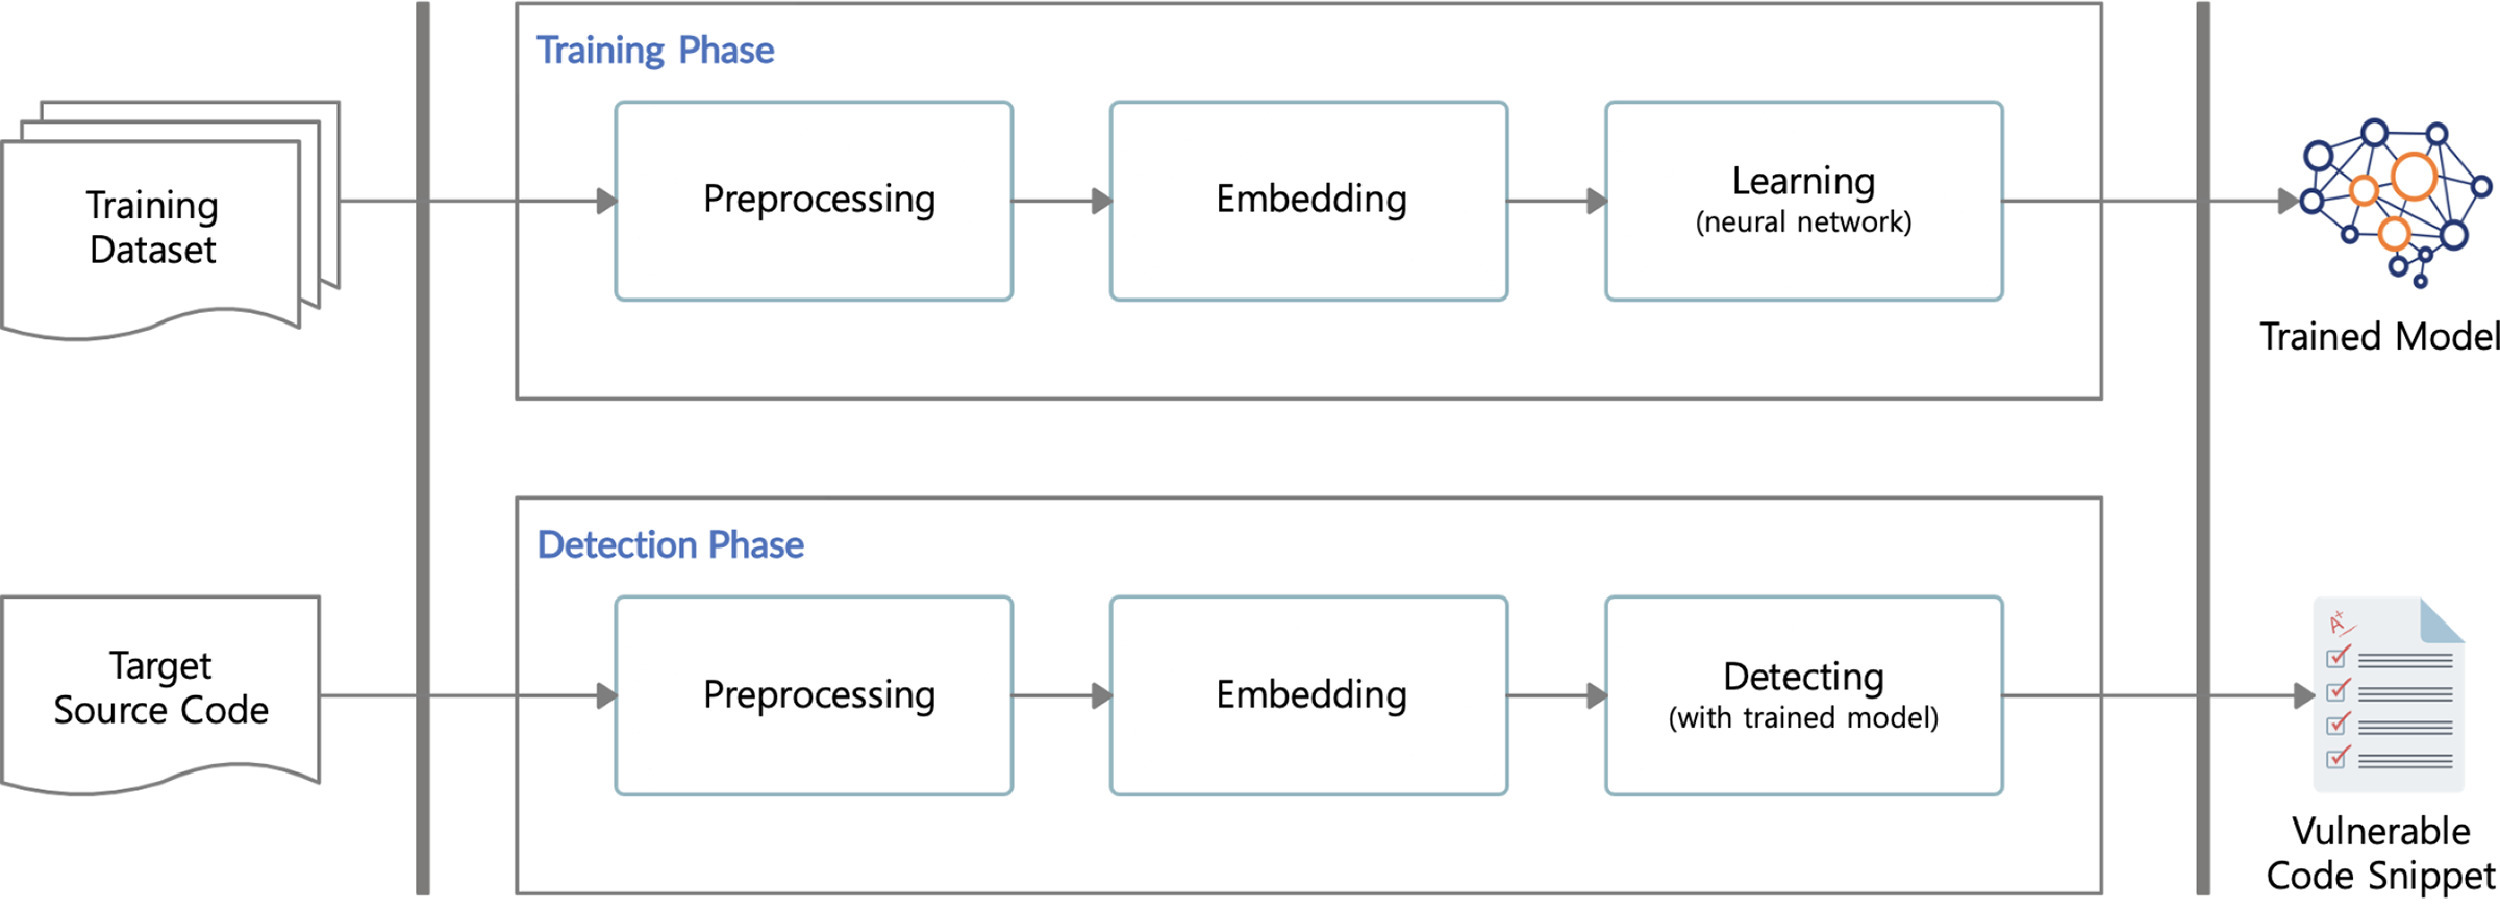
\includegraphics[width=\textwidth]{Algorithm}
	\caption{Deep-NC \cite{Vien2021}}
\end{figure}


\section{Results}

% Explain the experimental results in detail from your understanding (10 points)

\section{Advantages and Disadvantages}

% Discuss the advantages from your understanding (10 points)


% Discuss the disadvantages from your understanding (15 points)


\section{Improvements}

% Provide the specific ideas to improve the algorithm. General ideas are not allowed. (15 points)



\clearpage
\bibliographystyle{acm}
\bibliography{\jobname}
\end{document}